\chapter{序論}
\label{chap:introduction}

\section{背景}
\label{section:background}

組み込み向けデバイスの性能向上と低価格化により、身の回りの家具や家電をはじめとしたあらゆるものが
インターネットに接続し、協調して動作することで生活を豊かにするInternet of Things(IoT)が
普及しつつある。

Espressif Systemsによって開発されたESP32\cite{esp32}は、組み込み向けデバイスの中でも
比較的高性能かつ廉価なデバイスの一つである。
ESP32の主要な性能を以下に示した。

\begin{itemize}
  \item Xtensaアーキテクチャ 32-bit デュアルコアCPU 最大600MIPS
  \item 448KBのROMと536 KBのSRAM
  \item Wi-Fi 802.11 b/g/n 準拠
  \item Bluetooth 4.2 および Bluetooth Low Energy 準拠
\end{itemize}

ESP32はこのような豊富な計算資源と高度な無線接続機能を提供する一方で、そのソフトウェア開発環境は
柔軟であるとは言えない。
現在、ESP32向けのソフトウェア開発環境としてEspressif Systemsが公式にサポートしているのは、
以下の2通りの手段のみである。

\begin{itemize}
  \item C/C++でプログラムを記述し、ESP32ツールチェイン\cite{esp_toolchain}に含まれるGCCなどを用いてコンパイルする
  \item Arduino言語でプログラムを記述し、ESP32用の拡張\cite{esp_arduino}を導入したArduino IDE\cite{arduino_ide}を用いてコンパイルする
\end{itemize}

したがって、開発者がC/C++やArduino言語以外のプログラミング言語や、GCC以外のコンパイラ、
Arduino IDE以外のツールチェインといった異なる開発環境を使用する場合は、
非公式にESP32をサポートしているものを用いるか、自らESP32のサポートを追加で実装する必要がある。

ESP32における開発環境が限られているのは、ESP32が搭載しているXtensaマイクロプロセッサが用いる
Xtensa命令セットアーキテクチャ\cite{xtensa_isa}をサポートする開発環境が少ないためである。
翻って、x86やARMといったPCやサーバ向けに広く利用されている命令セットアーキテクチャにおける
ソフトウェア開発では、開発者には多くの開発環境の中から選択できる。
例えばプログラミング言語の選択という観点では、LLVMが機械語生成の対象としてサポートされている
ハードウェアであれば、LLVMを機械語生成に用いるプログラミング言語の全てが選択肢となりうる。
しかし、組み込み向けマイクロコントローラなど、用途が限定されているアーキテクチャの中でサポート
されているものは限られている\cite{llvm_matrix}。
Xtensaアーキテクチャも、LLVMによってサポートされていないものの一つである。

\section{本研究が着目する課題}

本研究では、\ref{section:background}節で述べた、ESP32が一般的でない命令セットアーキテクチャを
採用しているためにソフトウェア開発環境が限られている、という課題に着目する。
多くの開発環境がサポートしている別の命令セットアーキテクチャをESP32上で実行することができれば、
ESP32に向けたソフトウェア開発環境の選択肢を広げることができる。

\section{本研究の目的とアプローチ}

本研究の目的は、Xtensaアーキテクチャよりも多くの開発環境でサポートされているアーキテクチャ
向けにコンパイルされたプログラムを、ESP32上で実行することである。

そこで、本研究では仮想命令セットアーキテクチャとしてWebAssemblyを用いることを提案する。
また、実行形式としてWebAssemblyバイナリフォーマットを用いることを提案する。

本研究では、WebAssembly実行環境をESP32上に実装し、汎用的な開発環境を用いて生成された
プログラムを実行できることを示す。
これにより、仮想命令セットアーキテクチャとしてWebAssemblyを用いることで、ESP32の開発環境の
選択肢を広げられることを示す。

\begin{figure}[htbp]
  \caption{現状の開発フローと、本研究が目指す開発フロー}
  \label{fig:new_world}
  \begin{center}
    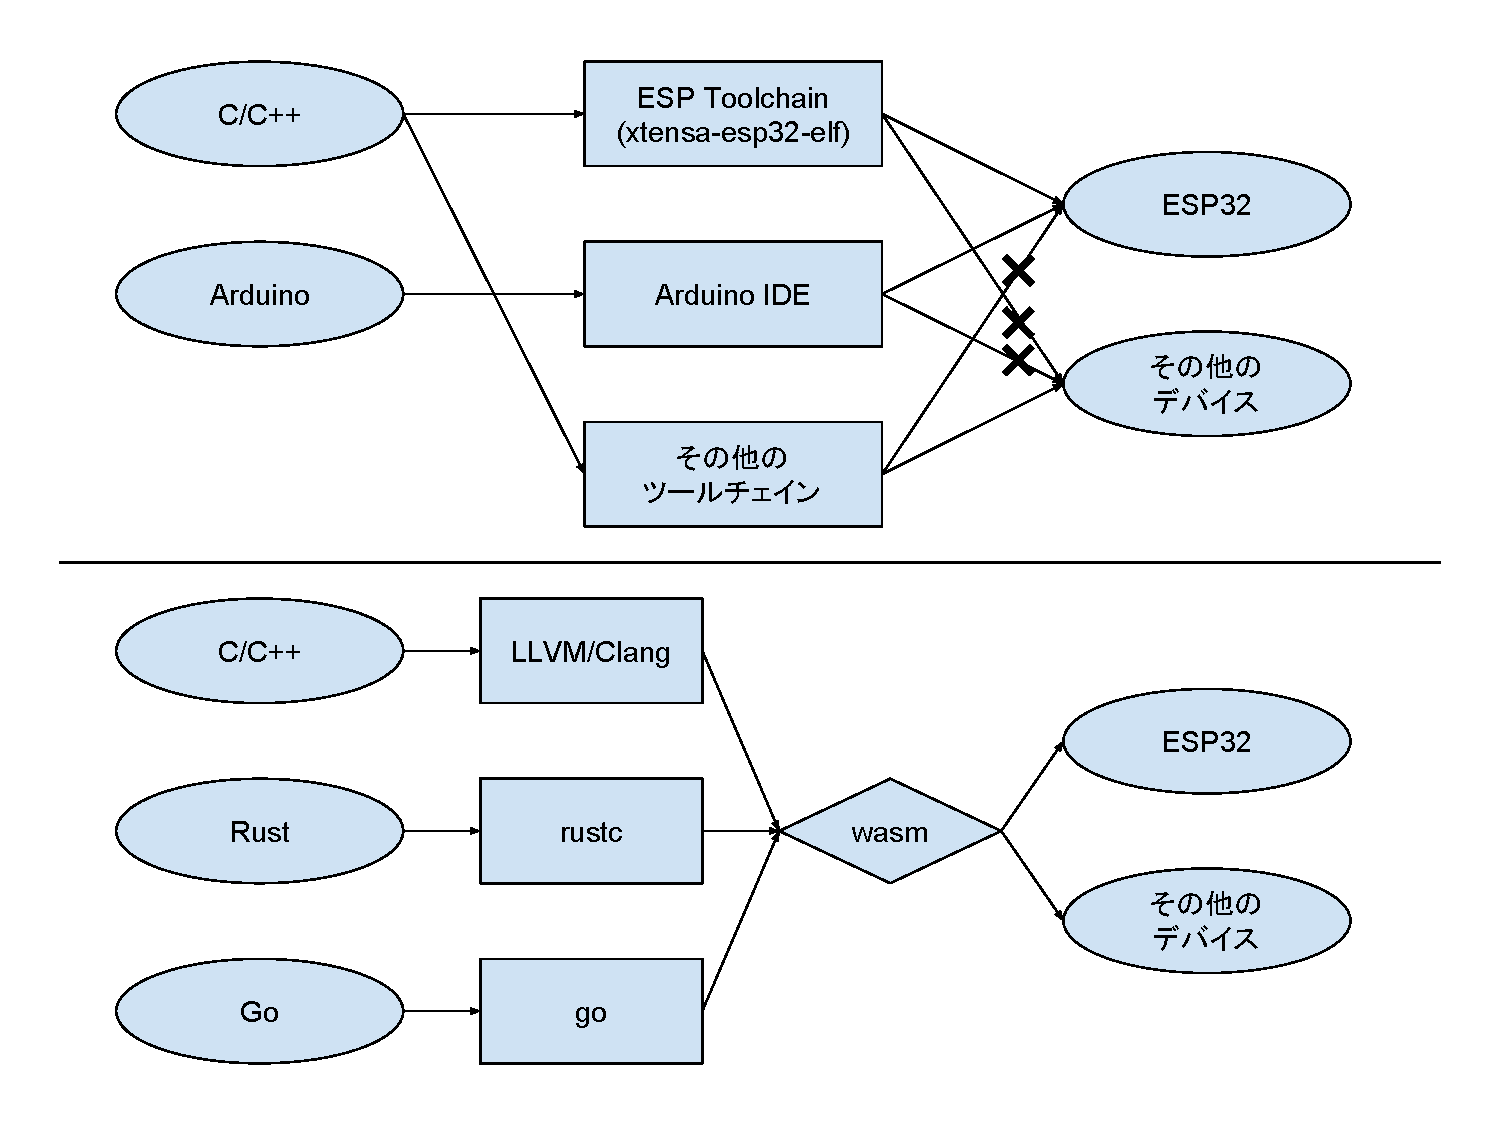
\includegraphics[bb=0 0 800 600,width=12cm]{img/new_world.pdf}
  \end{center}
\end{figure}

\section{本研究の構成}

本論文における以降の構成は次の通りである。

\ref{chap:related_works}章では、関連技術として〜。
\ref{chap:implementation}章では、本研究で実装するWebAssembly実行環境について、
設計と実装を示す。
\ref{chap:evaluation}章では、〜。
\ref{chap:conclusion}章では、〜。
